\documentclass[journal,twoside]{IEEEtran}

%% Citations
\usepackage{cite}
%\usepackage[sort&compress]{natbib}
%\bibpunct{[}{]}{,}{n}{,}{,}

%% AMS
\usepackage[cmex10]{amsmath}
\usepackage{amssymb,amsfonts}
\interdisplaylinepenalty=2500

%% Balance columns
%\usepackage{balance}

%% Better arrays
\usepackage{array}

%% Enumeration
\usepackage{enumerate}

%% Figures
\usepackage[pdftex]{graphicx}
\graphicspath{/Figures/}
\DeclareGraphicsExtensions{.png}
\usepackage[section]{placeins}

%% Fix some formatting issues
\usepackage{fixltx2e}
\usepackage{dblfloatfix}

%% Better cross-referencing
\usepackage[capitalize]{cleveref}

%% Newline for paragraphs instead of indenting
%\setlength{\parindent}{0in}
%\setlength{\parskip}{5pt plus 1pt minus 1pt}

\usepackage{threeparttable} % More control over tables

\usepackage{xcolor} % Use this for different colors -- useful for indicating what's changed since last review round
\newcommand{\changed}[1]{\textcolor{red}{#1}}
\renewcommand{\changed}[1]{#1} %Uncomment this to get rid of the red stuff
\newcommand{\rechanged}[1]{\textcolor{red}{#1}}
\renewcommand{\rechanged}[1]{#1} %Uncomment this to get rid of the red stuff
\newcommand{\rerechanged}[1]{\textcolor{red}{#1}}
%\renewcommand{\rerechanged}[1]{#1} %Uncomment this to get rid of the red stuff

%% correct bad hyphenation here
\hyphenation{op-tical net-works semi-conduc-tor}

% The paper headers
\markboth{IEEE Transactions on Components, Packaging, and Manufacturing Technology, Vol. ??, No. ??, Month ??, 20??}{Wahby \MakeLowercase{\textit{et al.}}: A Virtual Integration Platform for 2D and 3D IC Design Space Exploration}


\begin{document}
%% fix dashed lines for repeated author names in IEEE style bibliographies
%% NOTE: This requires some fiddling with the bibliography as well
\bstctlcite{IEEEexample:BSTcontrol} 

%% paper title
%% can use linebreaks \\ within to get better formatting as desired
%\title{\changed{Compact Modeling of Trends in 2D and 3DIC Power, Signal, and Thermal Performance}}
\title{\changed{A Simulation Tool for Rapid Investigation of Trends in 3DIC Performance and Power Consumption}}
%\title{\changed{3DVP: A Compact Tool for Investigation of Trends in 3DIC Performance and Power Consumption}}
\author{William~Wahby,~\IEEEmembership{Student~Member,~IEEE}, Li~Zheng, Yang~Zhang,~\IEEEmembership{Student~Member,~IEEE}, and Muhannad~Bakir,~\IEEEmembership{Senior~Member,~IEEE}%
	\thanks{\rerechanged{Manuscript received July 11, 2015; \changed{revised November 19, 2015; accepted November 21, 2015. Date of publication January ??, 2016; date of current version January ??, 2016. Recommended for publication by Associate Editor E.-P. Li upon evaluation of reviewers� comments.}}}%
	\thanks{This work was supported in part by the SRC GRC project 2254.001, and by the SRC Educational Alliance Intel Foundation Fellowship. The authors are with the School of Electrical and Computer Engineering, Georgia Institute of Technology, Atlanta, GA, 30332 USA. (emails: wwahby3@gatech.edu; lizheng@gatech.edu; steven.zhang@gatech.edu; muhannad.bakir@mirc.gatech.edu)}%
	\thanks{\rerechanged{Color versions of one or more of the figures in this paper are available online at http://ieeexplore.ieee.org.}}%
	\thanks{\rerechanged{Digital Object Identifier ???}} }%



\maketitle

%\IEEEpeerreviewmaketitle


%% =================================
%% ========== ABSTRACT =============
%% =================================
\begin{abstract}
In order to compare the costs and benefits of 2D and 3DIC technologies, a compact simulation tool for 3DIC system evaluation and
design space exploration is presented. The simulator is implemented in MATLAB, and is composed of several
modules, including a compact 3DIC wire length distribution,
a wire pitch and repeater insertion module, a 2D and 3DIC power supply noise
estimation module, and a finite difference thermal simulator.
The simulator is validated against published data for several commercial 2D processors at the 65nm, 45nm, and 32nm nodes.
In order to quantify the benefits of both 2D and 3D integration approaches, a 32nm CPU core is modeled and the impact of several
technology parameters, including interlayer dielectric (ILD) material, on-chip wire material, die thickness, 
and cooling solution are explored. The results suggest that 3D integration may provide a significant power reduction for the 32nm test case,
but more aggressive cooling solutions must be employed to maintain the same clock frequency due to the increased
areal power density of the 3D CPU. \changed{The simulation tool is available online at 
www.ece.gatech.edu/research/labs/i3ds.}
\end{abstract}

\begin{IEEEkeywords}
Three-dimensional integrated circuits, integrated circuit modeling, integrated circuit interconnections, power dissipation.
\end{IEEEkeywords}

%% =================================
%% ======== INTRODUCTION ===========
%% =================================
\section{Introduction}
\IEEEPARstart{E}{conomic} and physical challenges to transistor scaling are driving interest in 3D integration,
but uncertainty regarding the fabrication costs and system-level tradeoffs of 3D integration
complicate 3DIC design. Projections of 3DIC cost and performance are further impacted by the strongly-coupled
nature of communication, power delivery, and thermal management in 3DICs. The 3DIC
design space is complex, as 3DIC design encompasses a broad spectrum of possible design choices and integration
methodologies, ranging from 2.5D interposer-based integration all the way to finely-grained monolithic 
3DICs, as shown in \cref{f-3d-spectrum}, each with unique costs and strengths.
\begin{figure}[!tb]
	\centering
	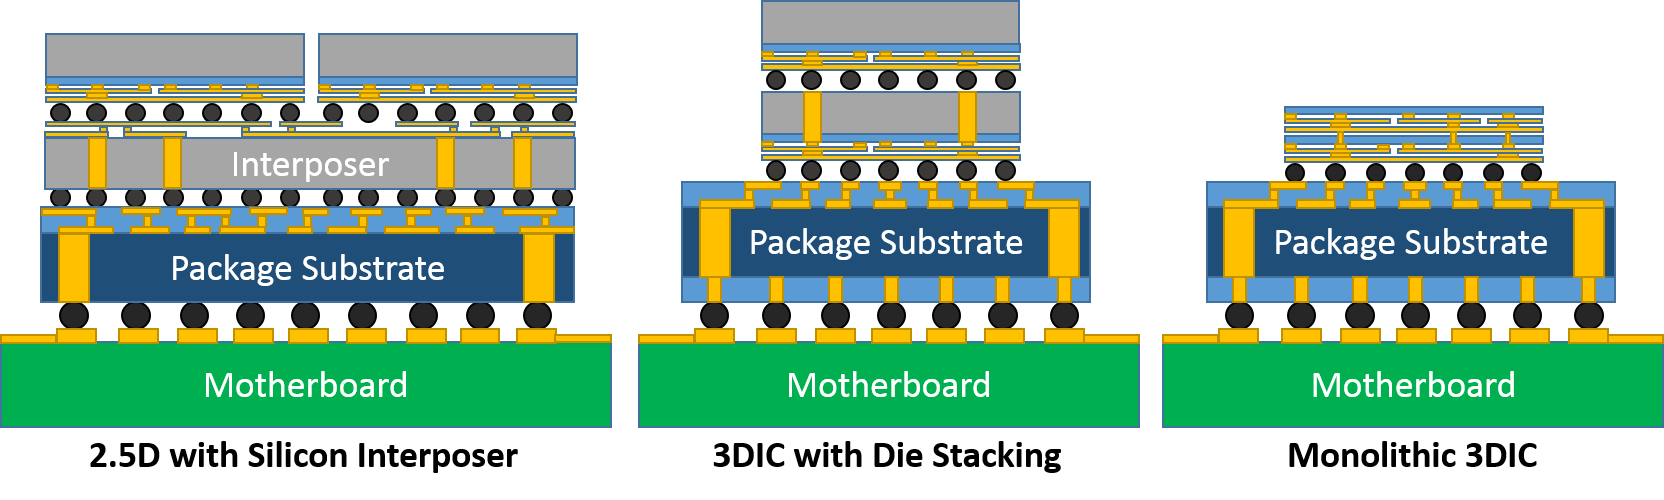
\includegraphics[width=3.5in]{Figures/spectrum_of_3d_4.png}
	\caption{There are many potential configurations for 3DICs, each with their own costs and advantages.
			Designers must manage the complexity of the 3DIC design space in order to achieve higher performance
			and lower cost systems.}
	\label{f-3d-spectrum}
\end{figure}
Additionally, different technologies must be evaluated for use in both 2D and 3DICs.
Low-k dielectrics can be used to reduce the parasitic capacitances in the wiring stack,
simultaneously improving RC delay and reducing the power consumption of the wiring network.
Alternate wiring materials are also being considered to improve the RC delay of on-chip interconnects,
as well as to reduce the impact of electromigration \cite{adelmann_alternative_2014}. 
Liquid cooling can be used to mitigate the thermal challenges
in high performance 3DICs\cite{tuckerman-high-performance-1981,zhang_within-tier_2013}. In order to understand when a 3D system
might have advantages over a 2D system, all of these factors must be modeled simultaneously.
\changed{Performing these coupled simulations with high fidelity is computationally intensive, however, rendering
thorough exploration of the 3DIC design space challenging.}
\changed{Compact tools have been developed to estimate 2DIC performance \cite{venkatesan-optimal-2001,sekar_intsim_2007}, but
no analog exists for 3DICs. Additionally, the existing 2D tools do not model power delivery or heat extraction, 
which are likely to be challenges for 3DICs.}


%The novel contribution of this work is the development of a compact tool capable of
%rapidly estimating the power consumption, simultaneous switching noise, and thermal profile
%of 2DICs and 3DICs.
%The aim of this work is to investigate trends in system performance and power consumption
%as materials, devices, and integration methodologies are varied.
%This simulation tool is intended to help answer what-if questions,
%to guide more precise investigations into the details of 3DIC physical design.

\changed{The novel contribution of this work is the development of a compact tool capable of rapidly simulating the
properties of 3DIC on-chip signal and power delivery networks.
The simulator estimates the power consumption, simultaneous switching noise, and thermal profile of 2DICs and 3DICs, 
and enables the investigation of trends in performance and power consumption
as materials, devices, and integration methodologies are varied.
The details of the on-chip wires, TSVs, power delivery network, and steady-state thermal profile
are all modeled in order to develop a self-consistent picture of the overall 3D system performance.
The simulator is intended to help answer what-if questions
and to guide more precise investigations
into the details of 3DIC physical design.}

\changed{The organization of this paper is as follows: 
in \cref{s-virtual-platform} the details of the models used and their interactions are presented;
in \cref{s-validation} the simulator is benchmarked against
wire pitch and TDP data from several commercial processors;
in \cref{s-2d-investigations,s-3d-investigations} the simulator
is used to investigate the impacts of advanced
technologies on a 32nm CPU core.}
Specifically, the impacts of the interlayer dielectric, wire material, and 3D stacking on the power consumption,
power supply noise, and metal layers required for routing are investigated.

\section{Simulation Framework} \label{s-virtual-platform}
The simulation platform consists of the following:
 \begin{enumerate}
	\item 3D wire length distribution which accounts for TSV area
	\item Metal layer pitch determination algorithms capable of handling alternate wiring materials
	\item An optimal repeater insertion scheme
	\item A power supply noise model for 3DICs
	\item A finite difference thermal module for analyzing the thermal impacts of 3D integration
\end{enumerate}

The simulation flow is shown in \cref{f-vp-flowchart}.
%\changed{The user first inputs high-level design parameters, including the target clock frequency,
%estimated logic activity factor (the fraction of transistors switching on any given clock cycle), transistor size and
%leakage parameters, wiring material, and expected die area and thickness.
%For 3D designs, the user must also specify the desired TSV diameter and aspect ratio, as well as the number of tiers
%used to implement the 3DIC.}
\changed{First, the distribution of 
wire lengths in the system is estimated, which is in turn used to determine the number of wiring tiers required for signal routing, 
the wire pitch on each tier, and the number of repeaters needed to meet the delay constraint.}
\changed{
In order to model the on-chip interconnects in a compact manner, the system is modeled as a homogeneous block
of randomly interconnected logic.
This assumption is commonly used with stochastic wire length models for rapid estimation of on-chip interconnect properties, at the cost of
reduced insight into fine-grained design details \cite{davis_stochastic_1998,joyner_impact_2001,sekar_intsim_2007}.
}
%
\changed{
In heterogeneous systems each block is modeled separately, 
and the results are assembled into an overall power density map of each tier in the design
to determine the thermal profile throughout the stack. In order to better predict the
performance of such systems, the method of \cite{zarkesh-ha_pin_1998} can be used to homogenize
a heterogeneous system.}
%\changed{
%Inter-block connections in heterogeneous designs are ignored, 
%as additional design-specific information is needed to determine their properties.
%Similarly, off-chip interconnects are ignored when simulating both homogeneous
%and heterogeneous designs, as additional design details would be needed for accurate simulation.
%}



\changed{Once the parameters of the on-chip interconnects are known, their power consumption can be estimated
%on-chip interconnect parameters are known, the on-chip interconnect power consumption can be estimated.
The transistor dynamic and leakage power is also calculated to determine the overall power requirements for the design.
The total power consumption is used in conjunction with the TSV and package pin resistance and inductance
to estimate the simultaneous switching noise in the power delivery network. Additional \rechanged{power pads and TSVs}
are inserted until the noise drops to acceptable levels.
At this point the tool checks that the total TSV area does not exceed a user-specified limit; 
if TSV demand outstrips available area, the TSV diameter is reduced and the interconnect and power modules are rerun.}

\begin{figure}[tb]
	\centering
	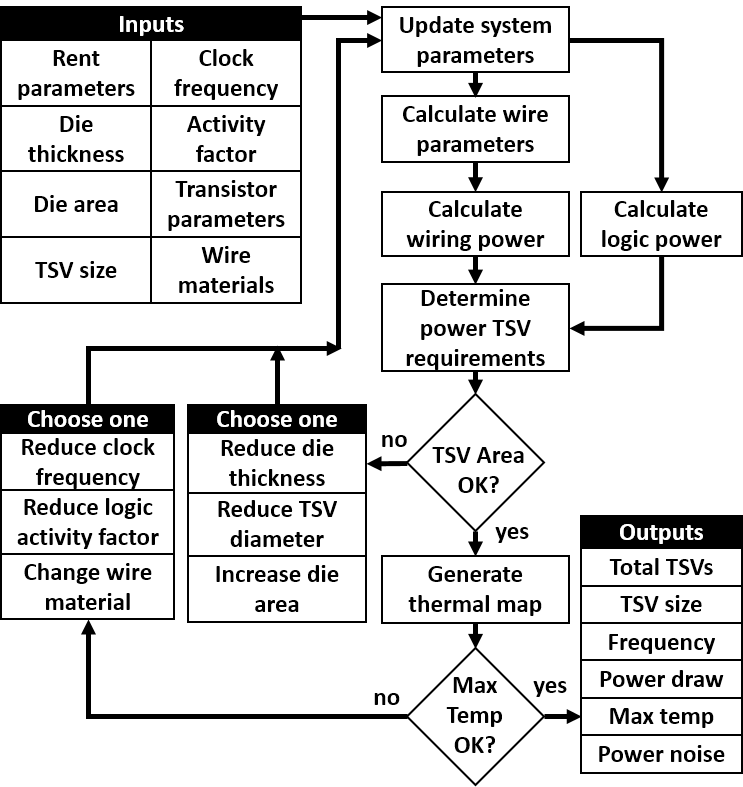
\includegraphics[width=2.75in]{Figures/vp-flowchart-4.png}
	\caption{Block diagram of the simulation platform execution flow.}
	\label{f-vp-flowchart}
\end{figure}

\changed{Once the design passes the TSV area check, the thermal module is used to estimate the maximum temperature in the 2D
or 3D design. In order to do this, the material parameters of the die, wiring tiers (including wires and interlayer
dielectric), TSVs, and interstitial layers are input into a finite difference thermal simulator, along with a heat transfer
boundary condition representing the heatsink. If the maximum temperature in the stack
exceeds a user-defined limit, the clock frequency is reduced and the previous modules are rerun until
the maximum temperature is sufficiently reduced. As alternate means of power reduction, the logic activity factor can also be reduced
or the wire or interlayer dielectric materials be modified.
The final design parameters are reported once the constraints on temperature and TSV area are satisfied. }

\rechanged{
The key limitations of this simulation platform are linked to the assumptions used to model the on-chip interconnects. % network.
Treating a design as a homogeneous block of randomly-interconnected logic allows
rapid simulation of the aggregate properties of the on-chip wires,
but limits visibility into the inner workings of the design.
Off-chip IO and interconnections between blocks in heterogeneous systems are also not modeled, as design-specific
information would be needed for accurate modeling. 
These omissions lead to underestimation of the system power, and limit the range of validity of
the simulator, but they also enable the consideration
of a wide range of system types without detailed design information.}



%% =================================
%% ========= Interconnects ============
%% =================================
\subsection{Interconnect modeling} \label{s-interconnect-modeling}
\changed{The on-chip interconnect network accounts for a significant fraction of the overall
power consumption in many logic designs \cite{sekar_intsim_2007}; accordingly, accurate determination of
the parameters of the on-chip interconnect network is crucial for developing reasonable estimates of
the overall power consumption and operation frequency of an integrated circuit. Specifically,
the number of metal layers used for wiring must be estimated, as well as the pitch of the wires on each level,
in order to determine the overall wiring capacitance, which is a key factor in the maximum wire delay and power consumption.}

Stochastic wire length models have been shown to be effective tools for the rapid prediction
of interconnect properties in 2DICs
\cite{davis_stochastic_1998,sekar_intsim_2007}.
and 3DICs
\cite{joyner_impact_2001},
but the impact of TSV-induced gate-blockage in 3DICs was not considered until \cite{kim_through-silicon-via_2009-1}
introduced a correction to account for finite TSV size. The method of \cite{kim_through-silicon-via_2009-1}
requires brute-force calculation, however, which is too computationally intensive for rapid simulation. 
To address this issue, a compact correction to the 
wire length distribution was introduced in \cite{wahby_wld_2013}, which is used in this work.
Once the wire length distribution is known, the wire pitch and number of metal layers are determined using a bottom-up wire scaling 
technique \cite{venkatesan-optimal-2001}, and a delay-optimal repeater insertion scheme 
is used to determine the size and number of repeaters required to meet timing constraints \cite{bakoglu_optimal_1985}.

The impact of surface scattering and grain boundary scattering on wire resistivity are incorporated into the wire sizing algorithm
with a combined Mayadas-Shatzke and Fuchs-Sondheimer (MS+FS) model, with
specularity of $0.55$ and backscattering probability of $0.43$ \cite{sun_surface_2010}.
The metal grain size is approximated as the smallest dimension of each wire.


%% =================================
%% ========= POWER ============
%% =================================

\subsection{Power supply noise modeling}
Power supply noise must be suppressed to ensure reliable system operation, but power delivery in 3DICs is 
complicated by the limited area available for routing power interconnects between tiers and by the additional
parasitic resistance and inductance of the TSVs used for power delivery. In order to determine the maximum allowable
TSV diameter, the number and size of the power delivery TSVs must be estimated.
%We use the analytic 3DIC power supply network models developed in \cite{zheng_novel_2014}
%to determine the simultaneous switching noise in the 3D stack and the number of power delivery TSVs.
%\changed{The periodicity of the power grid is used to extrapolate the frequency-domain behavior of a single power 
%delivery unit cell to determine the worst-case simultaneous switching noise in the system.}
%
\changed{The analytic 3DIC power supply model developed in \cite{zheng_novel_2014} is used to estimate the simultaneous switching noise (SSN)
in the 3D stack as a function of the number and size of the power delivery TSVs. The model uses the periodicity of the
power grid to extrapolate the worst-case SSN in the system from the detailed frequency-domain behavior of 
a single power delivery unit cell. Power is assumed to be delivered via a regular rectangular array of power and ground pads or TSVs
connected by planar power delivery wires. An inverse laplace transform is used to convert the frequency response of the power delivery network
into the temporal response, from which the worst-case noise can be easily extracted \cite{huang_power_2012}.}


%% =================================
%% ========= THERMAL ============
%% =================================
\subsection{Thermal modeling}
Thermal issues are one of the greatest challenges in 3DIC design.
In order to design a thermally robust 3D system, the relationships between device technology, system performance
area constraints, and packaging materials and technology must be explored.
To that end, we utilize a fast and accurate finite difference thermal model, \changed{described in \cite{xie_electrical-thermal_2011},
with a non-conformal meshing strategy described in \cite{zhang-thermal-2014}.}

\begin{figure}[tb]
	\centering
	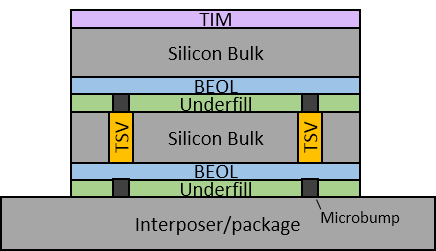
\includegraphics[width=1.75in]{Figures/thermal_config_no_bc_4.png}
	\caption{
		\changed{The geometry used in the thermal module. TSVs are individually meshed, in order to better capture the impact
		of 3D heat transport.}
	}
	\label{f-thermal-config}
\end{figure}


\changed{The thermal configuration considered in the simulation tool is shown in \cref{f-thermal-config}. One or more dice are assumed
to be stacked vertically atop an interposer (which may be either a conventional organic package substrate, or a silicon or glass
interposer). Each die is separated into three regions: 1) the bulk silicon, 2) the BEOL, which is modeled as the
volume-weighted average of the thermal conductivities of the wiring material and the interlayer dielectric, and 3) the underfill material
between each die. The power dissipated by each die is applied as an excitation at the boundary between the bulk silicon and the BEOL. 
TSVs are modeled within the bulk of any dice below the top die in the stack. Each external boundary is
modeled with a convective boundary condition; within-package boundaries are typically given a low heat transfer coefficient
of $5$ mW/m$^2$K, while the top and bottom surfaces are given higher values to reflect the cooling method used.}

\changed{The accuracy of this finite difference module was assessed in \cite{zhang-thermal-2014},} in which the performance of the finite difference scheme
was compared against finite element ANSYS models of the same structure. The finite difference model was found to match the ANSYS results with a maximum
error of 2.7\%.




%% =================================
%% ========= VALIDATION ============
%% =================================

\section{Validation} \label{s-validation}
The simulator was validated by comparing its predictions against published data for Intel processors ranging from the 65nm node
to the 32nm node
\cite{bai_65nm_process_2004,sakran_65nm_merom_arch_2007,mistry_45nm_process_2007,varghese_45nm_penryn_arch_2007,kumar_45nm_nehalem_arch_2009,packan_32nm_process_2009,kurd_32nm_westmere_arch_2010,yuffe_32nm_sandy_arch_2011}.
For each test case, the chip area, number of logic transistors, number of memory transistors, and size and shape
of the cores and memory blocks were gathered from published data. Logic cores were simulated with a Rent exponent of $0.6$,
while memory cores used a value of $0.4$, \changed{and GPUs were simulated with a Rent exponent of $0.5$} \cite{christie_interpretation_2000}.
\changed{Each block was simulated separately to determine the number and
pitch of metal levels required for routing and the total power consumption of each block.
The pitch and number of metal layers used for the overall design were then set by the block which required
the greatest number of wiring tiers (typically the CPU core). This information, along with the geometry and power requirements
of each block was then used by the thermal module to determine the maximum temperature in the system.}

\begin{table}[tb]
	\centering
	%\begin{tabular}{|c|c|c|c|c|c|}
	\caption{Comparison to actual data }
	\begin{threeparttable}
	\begin{tabular}{cccccl}
		\hline
						&			&	\multicolumn{2}{c}{Signal Wire Tiers}								&	TDP		&	\multicolumn{1}{c}{Predicted} \\
		Processor		&	Node	&	Actual											&	Predicted		&	(W)		&	\multicolumn{1}{c}{Power (W)} \\
		\hline \hline
		E6850			&	65nm	&	8												&	8				&	65		&	60.27 \changed{(-7.3\%)}	\\
		E8600			&	45nm	&	\changed{8}\tnote{2}							&	8				&	65		&	63.62 \changed{(-2.1\%)}	\\
		i7 880			&	45nm	&	\changed{8}\tnote{2}							&	7				&	95		&	105.56 \changed{(11.1\%)}	\\
		i7 680\tnote{1}	&	32nm	&	\changed{8}\tnote{2}							&	6				&	73		&	52.74 \changed{(-27.8\%)}	\\
		i7 2700k		&	32nm	&	\changed{8}\tnote{2}							&	8				&	95		&	91.80 \changed{(-3.3\%)}	\\
		\hline
	\end{tabular}
	\begin{tablenotes}
		\item[1] Multi-chip package with 32nm CPU die and 45nm gpu/support die.
		\item[2] Design has one additional global metal layer for power distribution.
	\end{tablenotes}
	\end{threeparttable}
	\label{t-validation}	
\end{table}


\begin{figure}[tb]
	\centering
	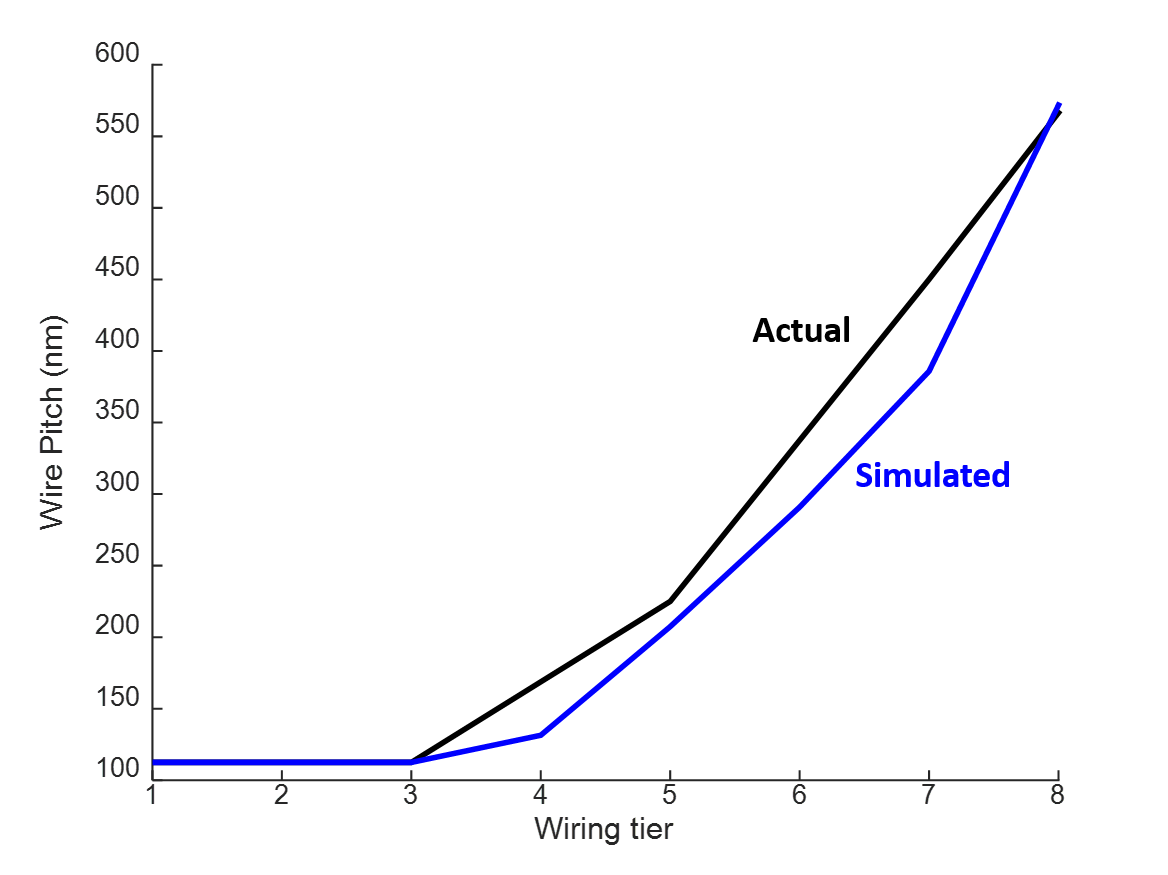
\includegraphics[width=3.5in]{Figures/sb_wire_pitch_2.png}
	\caption{
		Actual and expected wire pitch in a Core i7 2700k processor.
	}
	\label{f-sb-wire-pitch}
\end{figure}


The expected wire pitch, number of metal layers, power consumption, and
maximum junction temperature generated by the simulator have been compared in \cref{t-validation}. 
\changed{With the exception of the Core i7 680 test case, the tool shows reasonable agreement with the
published data for these processors. The 45nm and 32nm test cases all have a total of 9 metal layers, but in all cases
the wires on the top layer are sized very large and used for power and clock delivery, rather than signal routing.
Since the interconnect estimation
module is used estimate the size and pitch of signal wires only, the top metal layer in these designs is not counted
for the purpose of signal wire pitch validation. Instead, the upper wire tier is modeled in the power delivery simulation
module of the simulator, but without data on the
power noise margin and the number of power and ground pads used in these designs, detailed validation of the power
delivery module is not possible for these test cases.
In addition to the number of metal levels, the simulator accurately predicts
the wire pitch in each routing tier, as shown in \cref{f-sb-wire-pitch}.}



\changed{The simulator underestimates both the number of wiring tiers
and the overall power consumption for the Core i7 680 test case; this error could be due to the fact that the
Core i7 680 is the only design implemented as a multi-chip module (MCM), with a 32nm CPU die 
integrated with a 45nm GPU die in the same package.}
\changed{The simulator currently does not estimate the power required for inter-block communication in
heterogeneous systems. While this will affect the power estimates for all test cases, 
the power required for communication between the two
separate dice in the Core i7 680 is likely much larger than the power requirements for communication between GPUs and logic cores
integrated on the same die.}


%\changed{
%The value of this simulation platform lies
%in its ability to consider many different effects very rapidly 
%(a design scenario can be evaluated in several seconds on a laptop computer), 
%enabling the use of this tool for the investigation of the relative performance
%of many different technologies on a particular design.
%While the worst-case power error in these benchmarks is relatively high ($27.8\%$), 
%the typical error is low enough to answer what-if questions about 2D and 3DIC performance.
%In the subsequent sections the simulator is used in this manner
%to investigate the impacts of material, technology, and packaging innovations on the power consumption
%and performance of 2D and 3DICs.}

\rechanged{
The value of this simulation platform lies
in its ability to consider many different effects very rapidly,
%(a design scenario can be evaluated in several
%seconds on a laptop computer), 
%enabling investigation of the relative performance
%of many different technologies on a particular design.
enabling investigation of trends in the performance and power consumption of a reference design
over a wide range of technologies and configurations.
While the worst-case error in these benchmarks is relatively high ($27.8\%$), 
the typical error is much lower, and this level of accuracy is sufficient for the investigation
of power and performance trends in 2D and 3DICs.
In the subsequent sections the simulator is used in this manner
to investigate the impacts of material, technology, and packaging innovations on the power consumption
and performance of 2D and 3DICs.}

\section{2D: Impact of materials innovation} \label{s-2d-investigations}
One path towards increasing system performance is to achieve improvements in the wiring materials.
The permittivity of the interlayer dielectric (ILD) directly impacts the parasitic
capacitance of the on-chip wires,
which in turn impacts the wire RC delay and power consumption. Additionally, decreasing the RC delay
reduces the need for power-hungry repeaters.

In order to investigate the potential of ultra low-k (ULK) ILD materials, 
a 32nm Sandy Bridge Core i7 was simulated with a range of different
ILD permittivities, ranging from 3.9 (silicon dioxide), all the way down to 1 (vacuum).
Figure \ref{f-2d-materials-num-levels-ild} shows that the number of metal layers required to fully route
the Sandy Bridge processing core can be reduced from 8 to 6 if the relative dielectric constant
of the ILD material can be brought below 1.3.
\rechanged{Overall power consumption increases with}
ILD permittivity, as shown in \cref{f-2d-materials-power-consumption}, and significant power reductions
are possible with ULK materials. The power reduction comes from both a reduction in wire power,
as well as a reduction in the number and size of the repeaters needed to meet timing constraints.

\begin{figure}[tb]
	\centering
	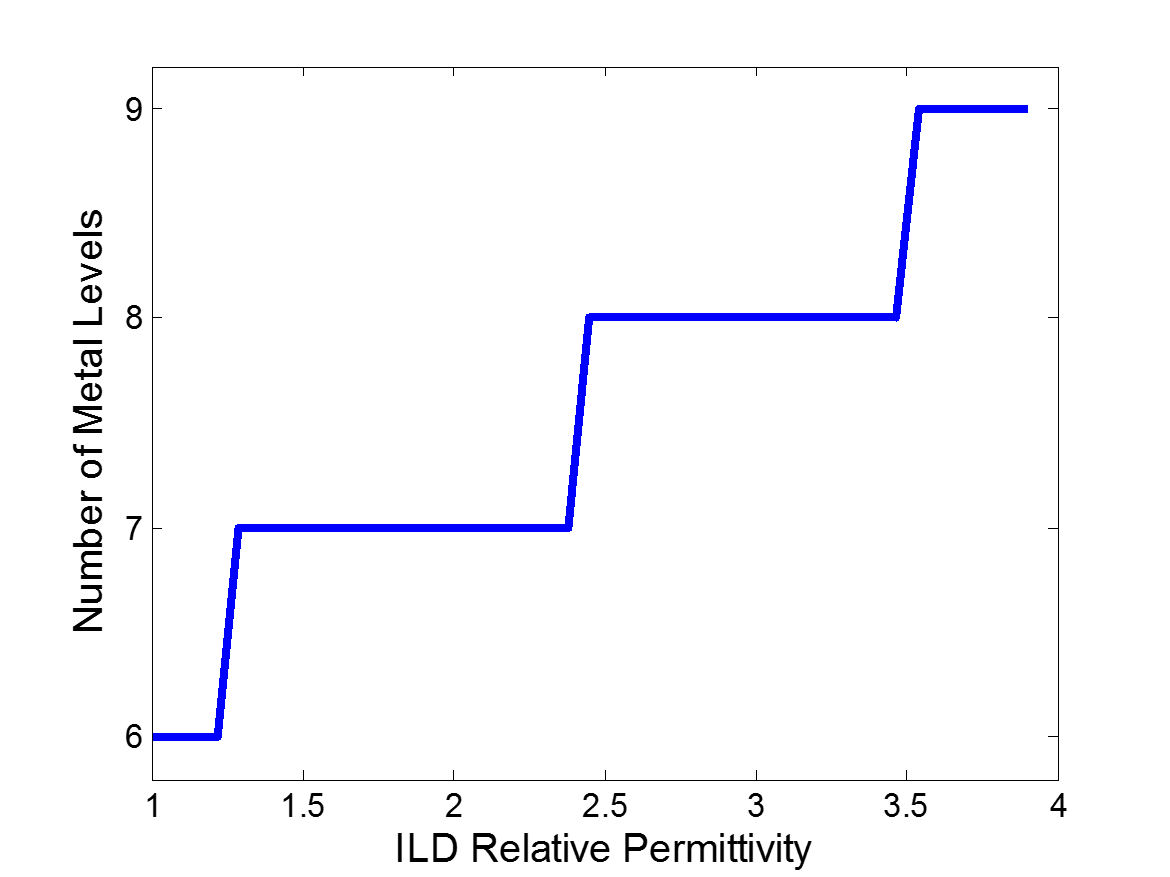
\includegraphics[width=3.5in]{Figures/sb_metal_layers_ild_eps_sweep_2.png}
	\caption{
		Impact of interlayer dielectric (ILD) permittivity on the number of metal layers required to route the wires in a Sandy Bridge Core i7 2700k.
	}
	\label{f-2d-materials-num-levels-ild}
\end{figure}

\begin{figure}[tb]
	\centering
	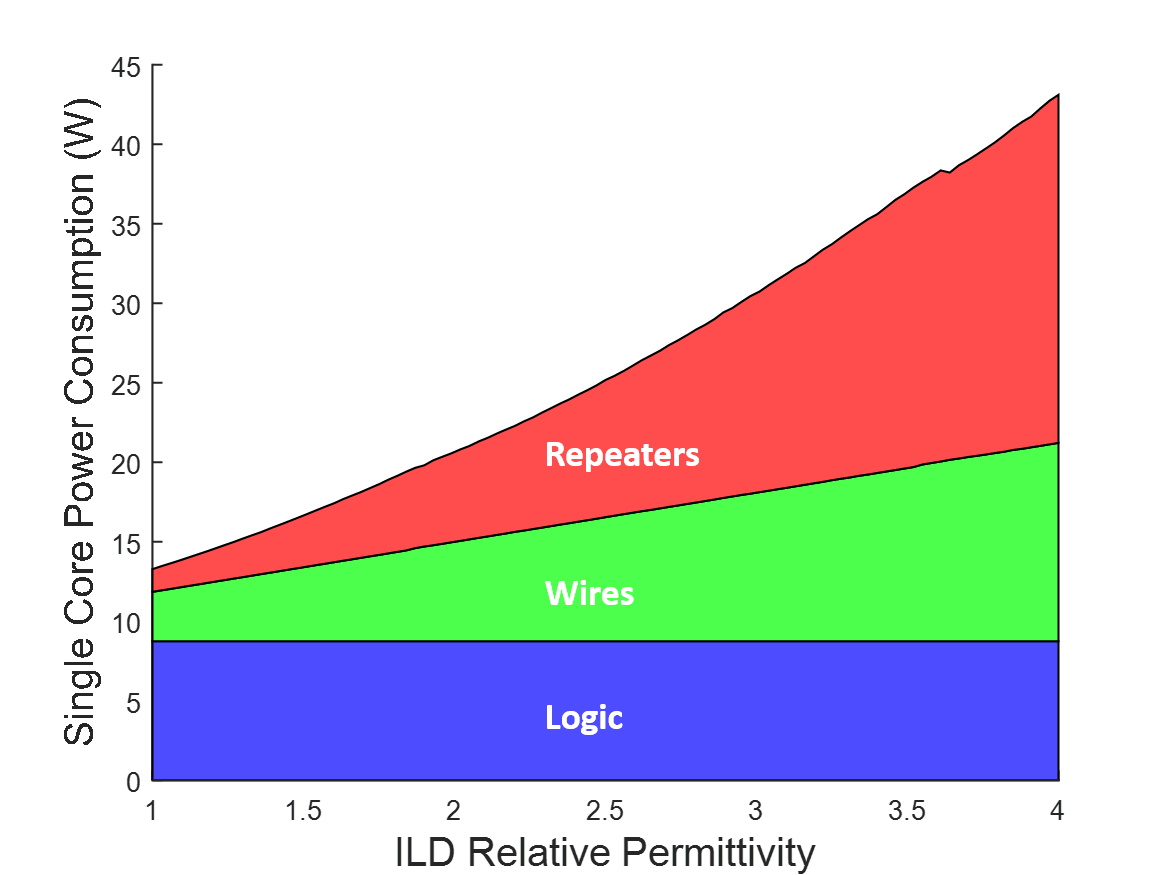
\includegraphics[width=3.5in]{Figures/total_power_sb2d_ild_permittivity_sweep_3.png}
	\caption{
		Impact of interlayer dielectric (ILD) permittivity on the power consumed by wires and repeaters in a Sandy Bridge Core i7 2700k core.
	}
	\label{f-2d-materials-power-consumption}
\end{figure}

As the critical dimensions of the smallest on-chip wires have decreased,
electromigration has become a reliability concern at advanced process nodes 
\cite{michael_electromigration_2003,tokei_reliability_2010}.
In order to address electromigration challenges at advanced process nodes, alternate materials may be required, 
potentially impacting signal performance, power consumption,
and the number of metal layers required to fully route a design \cite{adelmann_alternative_2014}. % Removed sankaran_exploring_2014
It is likely that only the lowest metal levels would use alternate materials \cite{oates-electromigration-2015}. 

To investigate the impact of alternate metals on routing,
a 7nm Sandy Bridge CPU test case was constructed by scaling \rechanged{down} the gate pitch, 
minimum wire pitch, transistor size, and all other lengths in the 32nm Sandy Bridge
by a factor of 4.57X (32/7). Two 7nm test cases were considered: \textit{7nm A}, in which all wires are composed of an
alternate material, and \textit{7nm B}, in which only wires thinner than 25nm are replaced by the alternate material.
The bulk resistivity of the alternate wiring material 
in both the 32nm and 7nm test cases was swept from 10 $\Omega$nm (slightly lower than bulk Ag), to 60 $\Omega$nm 
(slightly higher than bulk W).
%For simplicity, the specularity and reflection
%parameters of the alternate material are not modified.
As can be seen in \cref{f-2d-materials-num-levels-rho-7nm}, higher resistivity metals can significantly
increase the number of metal levels required for signal routing, but this effect can
be mitigated by restricting the use of alternate metals to the lowest wiring tiers.
Since the greatest numbers of wires are routed in the lowest tiers, small changes to their dimensions
can have large impacts on the wiring stack.

\begin{figure}[tb]
	\centering
	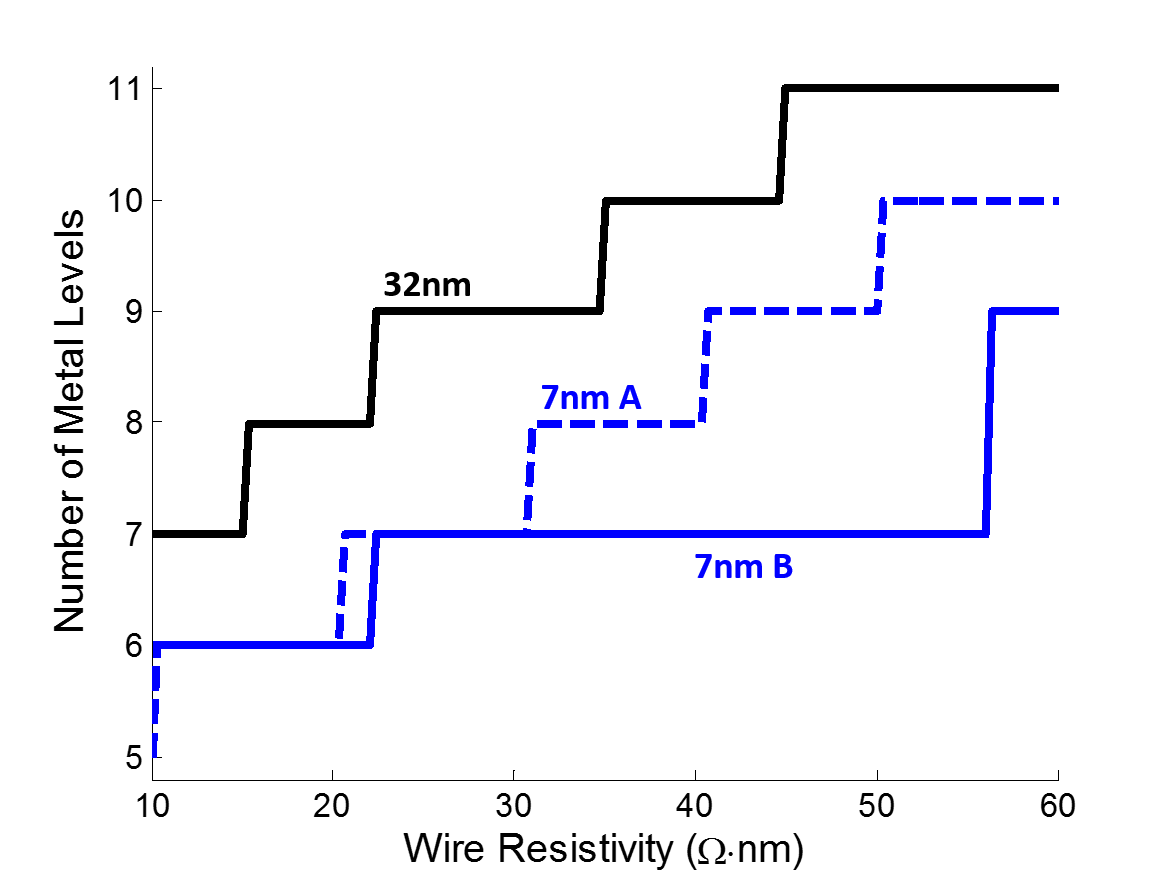
\includegraphics[width=3.5in]{Figures/sb2d_32nm_vs_7nm_alt_metal_comparison.png}
	\caption{
		Impact of wire resistivity on the number of metal layers required to route the wires in a Sandy Bridge CPU. Three cases are
		considered: a) a 32nm Sandy Bridge core; b) 7nm A, a hypothetical
		7nm Sandy Bridge core; and c) 7nm B, in which only wires with width below 25nm are modified.
	}
	\label{f-2d-materials-num-levels-rho-7nm}
\end{figure}



\section{3D: Power reduction without exotic materials} \label{s-3d-investigations}

\subsection{Reducing power consumption}
Implementing a design in 3D can greatly reduce the average length of the on-chip interconnects,
leading to reductions in the average delay and power consumption of the signaling network \cite{joyner_impact_2001}.
In order to examine the impacts of 3D integration, a single 18.5mm$^2$ CPU core from a 32nm Sandy Bridge Core i7 2700k
is examined throughout this section.
Unless otherwise noted, we assume a TSV aspect ratio of 20:1, and require that the TSVs use
less than 10\% of the total die area. Typically, 3DIC designs limit the TSV area to 1\% or less
to minimize the cannibalization of active area, but we have relaxed that limit here for illustrative purposes.
In order to examine the impacts of 3D integration, a single CPU core from a 32nm Sandy Bridge Core i7 2700k
is examined throughout this section. We consider a scenario in which logic gates and blocks can be placed on
any tier, and in which TSVs are used as point to point interconnects.
The core is assumed to be partitioned into $N$ equal pieces, which are then stacked vertically.

Significant power savings can be obtained by moving to a 3D design, as shown in \cref{f-sb-power-vs-tiers-ild},
though the power reduction comes at the cost of increased areal power density, ultimately placing more
stress on the heat sink. The design implications of the increased power density of 3DICs will be discussed further
in \cref{s-3D-thermal}. It is important to note that 3DICs reduce the on-chip communication power, fundamentally 
improving the 
energy efficiency of the system, as can be seen in \cref{f-sb-comm-power-fraction}.

\begin{figure}[tb]
	\centering
	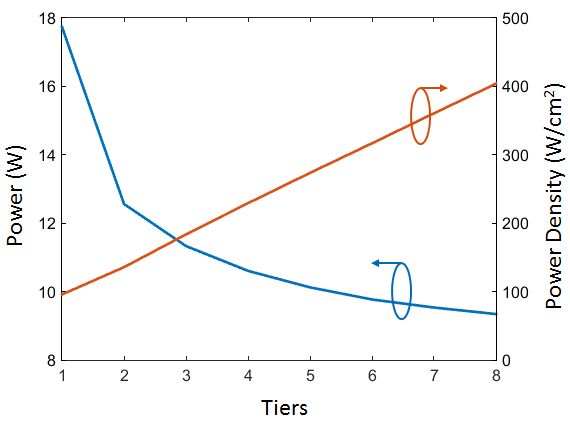
\includegraphics[width=3.5in]{Figures/sb3d_power_and_pdens2.png}
	\caption{Impact of block folding on power consumption and power density of a single 32nm Sandy Bridge core.}
	\label{f-sb-power-vs-tiers-ild}
\end{figure}

\begin{figure}[tb]
	\centering
	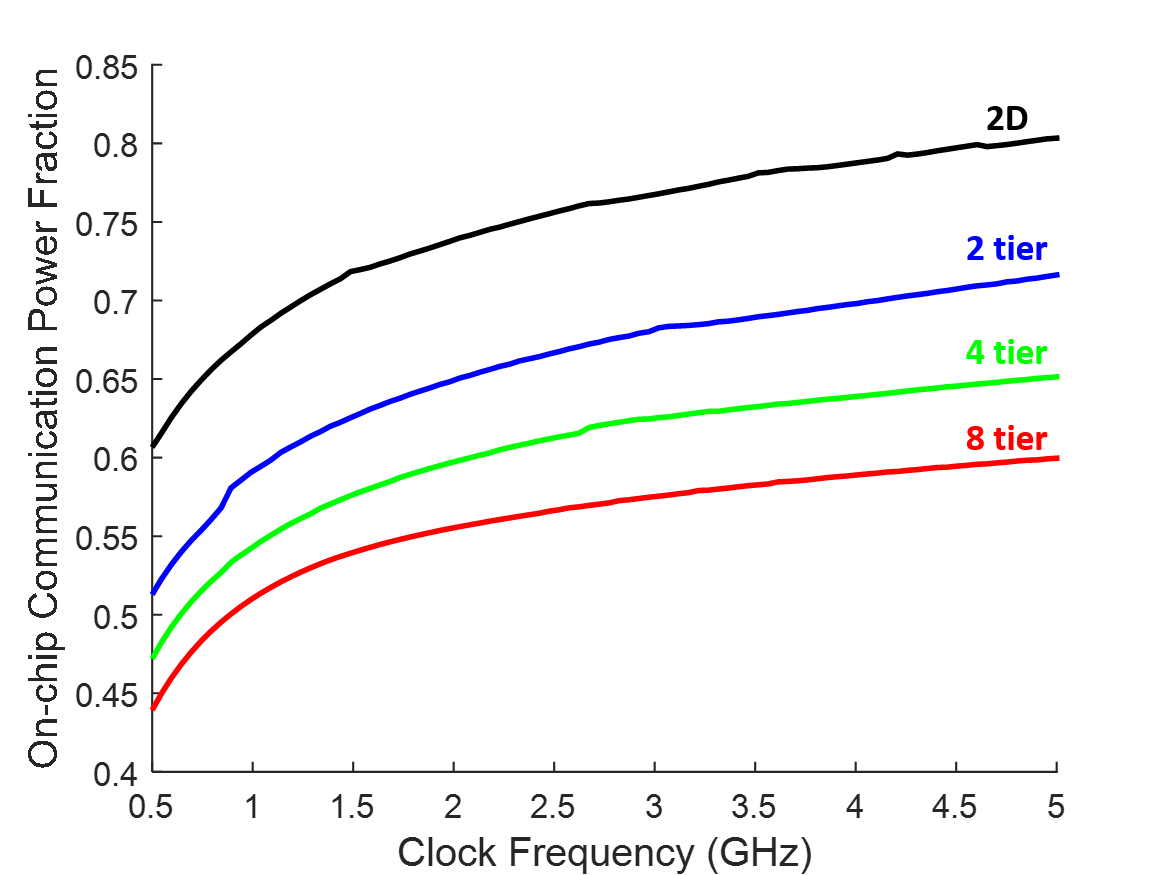
\includegraphics[width=3.5in]{Figures/sb3d_comm_power_fraction_4.png}
	\caption{Fraction of power consumed for on-chip communication as a function of 3D configuration and operating frequency.}
	\label{f-sb-comm-power-fraction}
\end{figure}


In order to fully route a 3DIC, space must be allocated on each tier for TSVs. Since TSVs consume space
that could be used for logic, it is desirable to minimize the fraction of chip area 
consumed by TSVs. TSV diameter can be reduced by either increasing the TSV aspect ratio or by die thinning.
Thicker logic tiers are attractive due to their higher mechanical stability, but they reduce the wire length advantages of 3DICs. 
TSVs are typically limited to diameters of 5-10${\mu}m$ and aspect ratios between 5-20:1 
\cite{lau_evolution_2011,zhang_within-tier_2013}.
%
The impact of die thickness on 3DIC power consumption is examined in \cref{f-sb-wire-power-thickness}.
In order to realize the greatest power reduction from 3D integration, the active layers should be
as thin as possible\rechanged{, to maximize the number of long wires that can be shortened by block folding.}

\begin{figure}[tb]
	\centering
	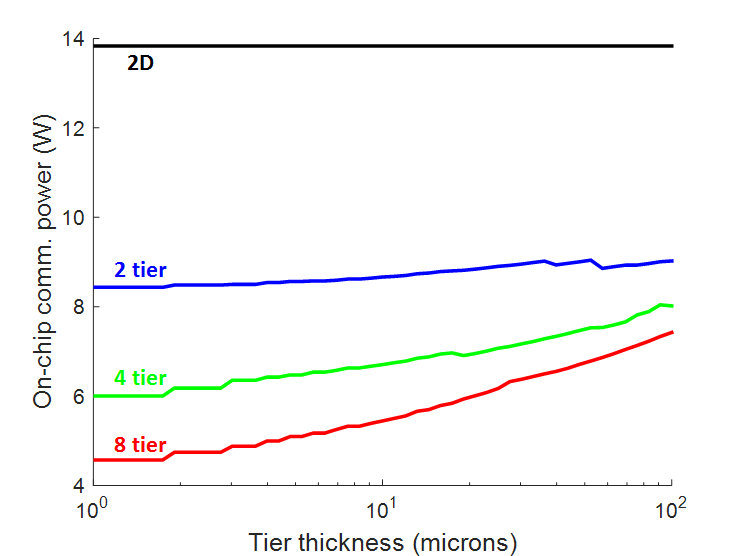
\includegraphics[width=3.5in]{Figures/sb3d-comm-power-vs-thickness_3.png}
	\caption{Impact of die thickness on power consumed by wires and repeaters in a single 32nm Sandy Bridge core implemented in 3D.}
	\label{f-sb-wire-power-thickness}
\end{figure}



\subsection{Power Delivery}
Power delivery in 3DICs is challenging, as a high performance 3DIC may have a significantly
higher areal power density than an equivalent 2D chip, while simultaneously having less space available for
routing power delivery resources. Additionally, power must be delivered to each tier
through TSVs, increasing the parasitic resistance and inductance of the power delivery network.
The number of power connections required by each tier is determined by the power draw and power density 
of the system,
which depends upon the dielectric properties and the substrate thickness (for 3DICs).
Both 2D and 3D systems benefit from the use of ULK interlayer dielectrics, and 
the use of thin substrates in 3D configurations can further reduce the demands on the power supply network.

In order to explore these effects, the Sandy Bridge test case was simulated with several substrate thicknesses and 
dielectric permittivities, in order to determine the number of power delivery pads or TSVs needed to reduce
the simultaneous switching noise to below 15\% of the nominal supply voltage. The results are presented in \cref{f-3d-psn-ild-tiers}.
For two-tier stacks only a slight increase in power TSVs is observed over the 2D case, but
the eight-tier implementation requires roughly an order of magnitude
more power connections than the 2D design. The ILD permittivity has a strong impact on the power delivery requirements,
as it directly affects the power consumption of the on-chip communication network. The thickness 
of the 3DIC logic tiers is not a limiting factor for 2-tier designs, but 4- and 8-tier designs can realize nearly as much benefit
from die thinning as from ULK dielectrics\rechanged{, due to the reduced power consumption of thin-tier 3DICs (\cref{f-sb-wire-power-thickness}).}

\begin{figure}[tb]
	\centering
	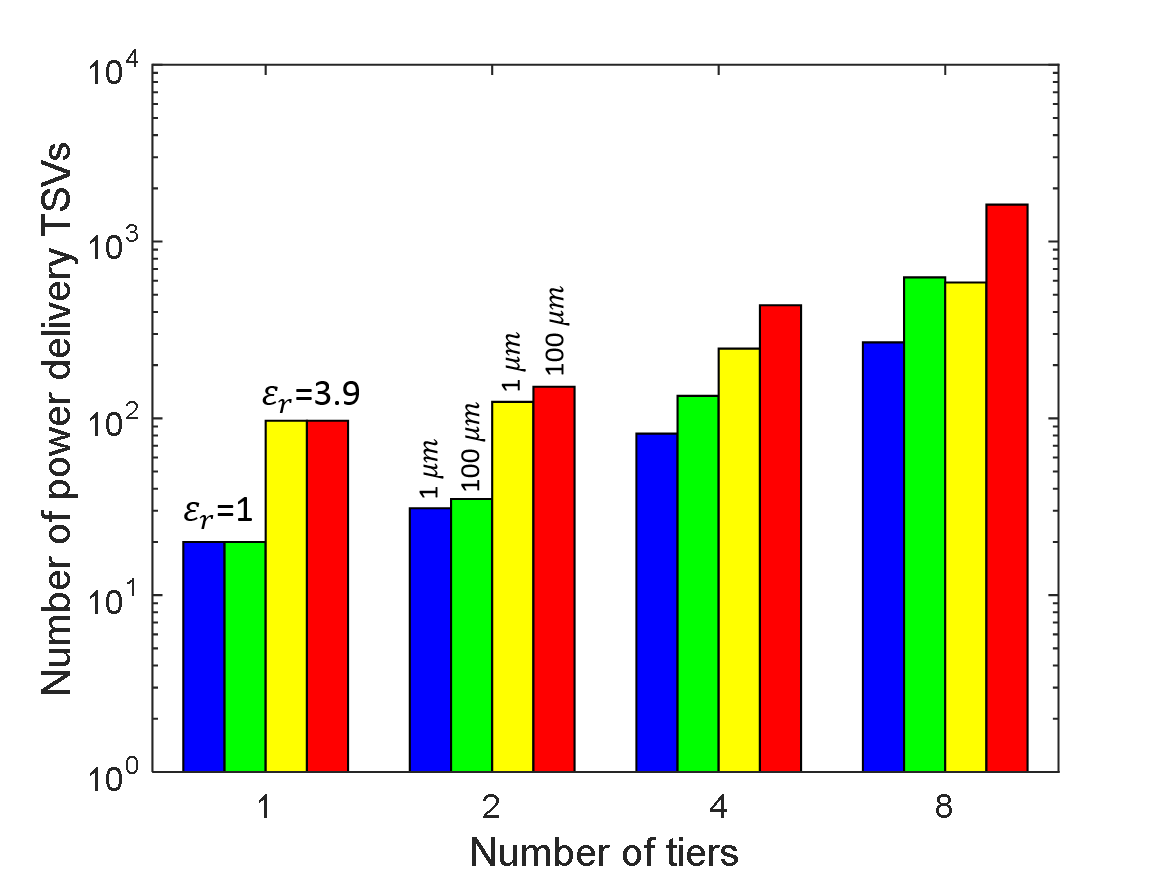
\includegraphics[width=3.5in]{Figures/sb3d_psn_vs_ild_and_tiers_vacuum_vs_sio2_3.png}
	\caption{
		Impact of interlayer dielectric material, substrate thickness, and 3D 
		integration on power pad/TSV requirements in a 3D Sandy Bridge CPU core.
	}
	\label{f-3d-psn-ild-tiers}
\end{figure}

\begin{figure}[tb]
	\centering
	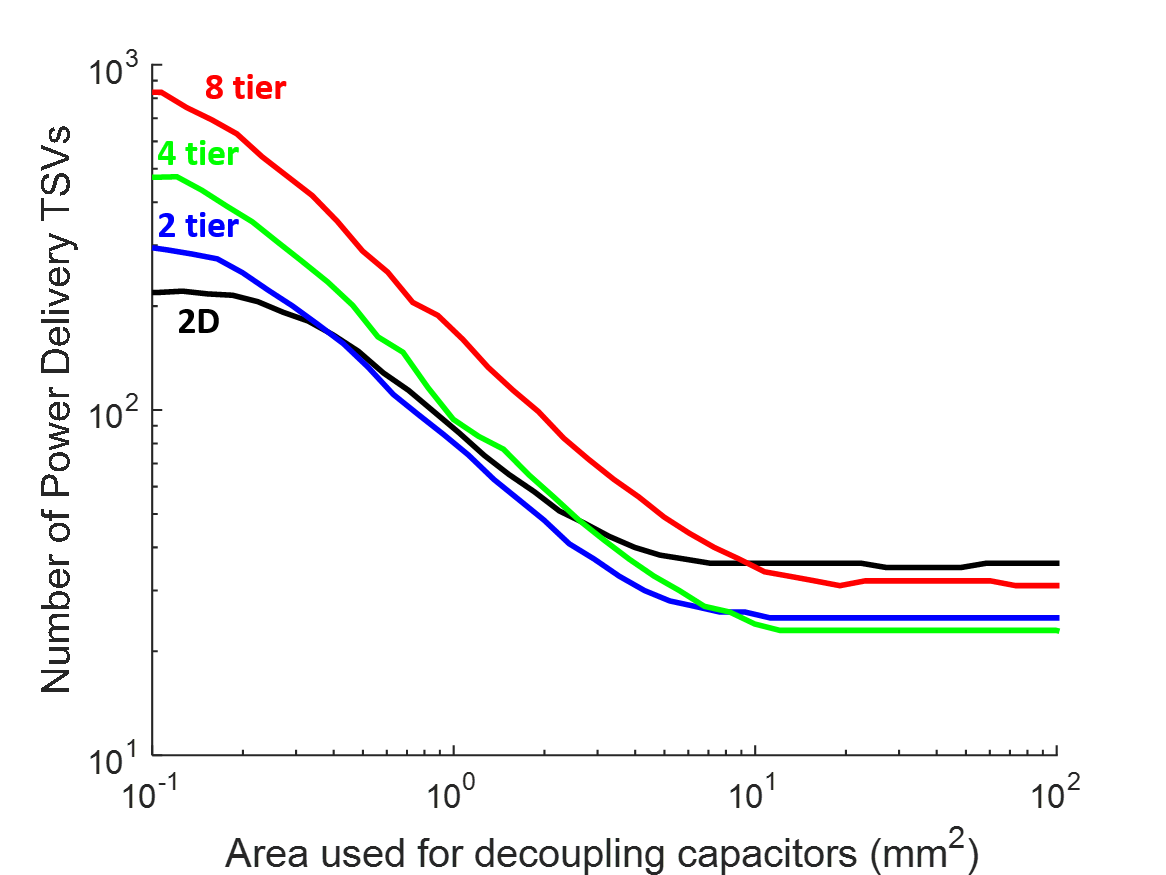
\includegraphics[width=3.5in]{Figures/sb3d_psn_tiers_and_decap__substrate_10um__tsvs_10um_3.png}
	\caption{
		Power TSV requirements for a single Sandy Bridge core as a function of 3D configuration and
		area allocated for decoupling capacitors.
		}
	\label{f-sb-psn-decap-10um}
\end{figure}

Another method to reduce power supply noise is to integrate decoupling capacitors onto the die
to compensate for the inductance of the power delivery network. While this practice can improve
power quality, it also sets up a tradeoff between utilizing die area for logic and power delivery.
To explore this tradeoff, the 32nm Sandy Bridge test case was simulated in 2D and 3D configurations with
varying amounts of silicon area allocated for decoupling capacitors. The power TSV diameter is assumed to be 10 ${\mu}m$ and the thickness of each die in the 3D stack is assumed to be
10 ${\mu}m$ \changed{to investigate the potential of extreme die thinning. While handling thinned wafers can be challenging,
alternate integration schemes in which wafers are bonded and subsequently thinned could enable the stacking of such thin layers
without the need for modified wafer handling processes \cite{patti-three-dimensional-2006}. Alternately, monolithic 3DIC fabrication
techniques could enable designs with extremely small intertier distances \cite{vinet-monolithic-2014}.}
\rechanged{For simplicity, the impact of electromigration on power delivery TSVs is ignored.} As can be seen in \cref{f-sb-psn-decap-10um}, increasing the decoupling
capacitance can significantly reduce the number of power pads or TSVs, but achieving high decoupling capacitance densities could be challenging. 
\rechanged{Even with the use of decoupling capacitors, a more stringent lower bound on power TSV number may be set by
the need to keep the current density carried by each TSV low enough to avoid electromigration.}





\subsection{Thermal management} \label{s-3D-thermal}
Thermal management is a key challenge for 3DICs.
While the total power dissipation of an IC is expected to decrease as the system is partitioned into increasing numbers of layers 
(as shown in \cref{f-sb-power-vs-tiers-ild}),
the areal power density will still increase as tiers are stacked atop one another,
leading to increased stress on the cooling system.
In order to quantify the thermal impact of 3D stacking, the performance of a single 32nm Sandy Bridge CPU core is examined 
\changed{in both 2D and 3D configurations, and with both air-cooled and \rechanged{liquid-cooled} heat sinks. 
\rechanged{In all cases the heat sinks are located on the back side of the top die.}
The air-cooled heat sink has a heat transfer coefficient of $1.83$ W/cm$^2$K and the fluidic heat sink
has a heat transfer coefficient of $4.63$ W/cm$^2$K \cite{zhang-micropinfin-heat-sink-2013}.
Boundaries internal to the package are assigned a heat transfer coefficient of $0.005$ W/cm$^2$K. The
thermal conductivities used for the materials in the stack are presented in \cref{t-thermal-materials}.}

\begin{table}[tb]
	\centering
	\caption{Material parameters used for thermal simulation}
	\begin{tabular}{cccccl}
		\hline
%						&	Thermal \\
		Material		 & Thermal Cond. (W/mK) \\
		\hline
		\hline
		Silicon			&	149 \\
		Copper			&	400 \\
		Underfill		&	0.3 \\
		Microbumps		&	60	\\
		Silicon Dioxide	&	1.38 \\
		\hline
	\end{tabular}
	\label{t-thermal-materials}	
\end{table}

\begin{figure}[tb]
	\centering
	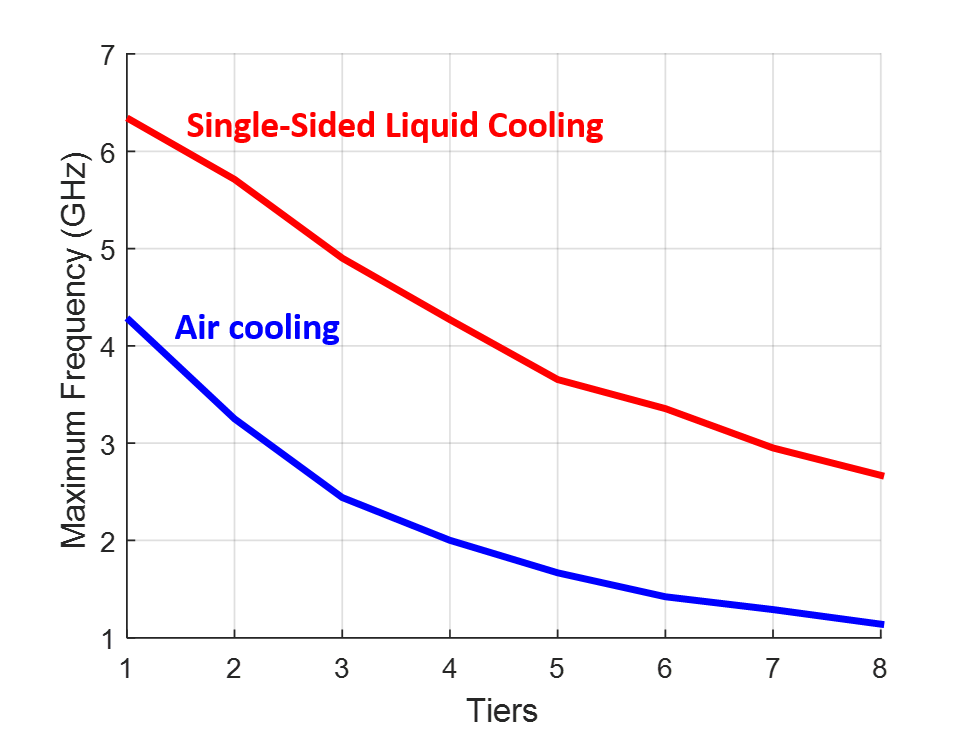
\includegraphics[width=3.5in]{Figures/SB3D_max_frequency__air_vs_water_cooling_2.png}
	\caption{
		Maximum clock frequency of 2D and 3D 32nm Sandy Bridge CPU cores limited to 90$^\circ$C under air cooling (blue)
		and \rechanged{liquid} cooling (red).
		}
	\label{f-sb3d-freq-vs-tiers}
\end{figure}



The CPU core was simulated in each configuration to find 
the maximum operating frequency which could be maintained while keeping the stack below 90$^\circ$C.
\changed{In order to focus on the thermal aspects of 3D stacking we assumed that the system was thermally-limited, and ignored other
factors which could limit the operating frequency of the chip, such as clock distribution.
The power consumed by the cooling solution is ignored, in order to isolate intrinsic die-level
effects from the details of the heat sink.}

As can be seen in \cref{f-sb3d-freq-vs-tiers}, the maximum frequency decreases steadily as the CPU is folded across
more tiers, as the increased power density (\cref{f-sb-power-vs-tiers-ild}) of the
system increases the strain on the cooling system.
\changed{In all cases, the microfluidically-cooled cores can run faster than the air-cooled cores.}
\changed{It is important to note that the configuration considered here represents the most thermally challenging 3D integration scenario:
the stacking of high performance logic. 
\rerechanged{Systems which are not thermally-limited will be able to take greater advantage of 3D integration to increase performance and
decrease power consumption.}
With a more aggressive cooling solution the \rerechanged{thermally-limited} logic core considered here can be folded over up
to four tiers while still achieving performance parity with an air-cooled 2D implementation.
\rechanged{Additionally, microfluidic coolers could be integrated into each die in the stack to further
reduce the temperature of the stack.}}
%\rerechanged{It is important to note that systems systems which are not thermally-limited will be able to take even greater advantage of 3D integration
%to increase performance and decrease power consumption.}




%% =================================
%% ========= CONCLUSION ============
%% =================================

\section{Conclusions}
A compact simulation tool for 2D and 3D IC pathfinding was developed and used to examine the impacts of 
advanced technologies on system performance. The tool incorporates 
models for signal delivery, power supply noise, and thermal performance in 2D and 3D ICs,
and was validated against wire pitch and power consumption data for recent commercial microprocessors.
%The impacts of low-k dielectrics, and 3D integration on the performance, power consumption,
%and power delivery requirements of a 32nm processing core were examined, and a 7nm version of the same processor
%was simulated to determine the impact of alternate wire materials on the number of metal levels required for routing
%at advanced process nodes.
\changed{
The simulation results suggest that high performance 3DICs may require large numbers of power delivery TSVs,
due to the TSV parasitics introduced into the power delivery network, as well as the
increased power density of the 3D cores. Die thinning and low-k dielectrics are expected to
be effective tools for reducing the power consumption and power TSV requirements of high performance 3DICs.
The results suggest that 3DICs should exhibit greater energy efficiency
than their 2D counterparts, though \rerechanged{thermally-limited} 3D designs may require more aggressive cooling solutions.}
%to achieve
%performance parity. }



\section*{Acknowledgments}
The authors gratefully acknowledge the support of the Semiconductor
Research Corporation Global Research Collaboration (task ID 2254.001),
as well as the SRC Educational Alliance Intel Foundation Fellowship.

%% Fiddle with this to manually align columns on last page
%\enlargethispage{-1.0in}


%% Include bibliography
\bibliographystyle{IEEEtran}%_local}

% Use this to manually decrease the effective page size to balance the bibliography columns.
%May not work in all IEEE modes.
%\IEEEtriggercmd{\enlargethispage{-1.0in}} 

%% Use this to break the references at a particular reference number (don't use with enlargethispage)
%\IEEEtriggeratref{26}

% Start the bibliography!
\bibliography{references}

\vspace{-0.3in}

\begin{IEEEbiography}[{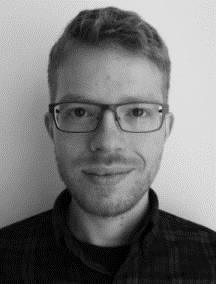
\includegraphics[width=1in,height=1.25in,clip,keepaspectratio]{Figures/bio-will.png}}]%
{William Wahby}
(S13) received the B.S. and M.S. degrees in electrical and computer engineering from the
University of Illinois at Urbana Champaign in 2007 and 2009, respectively. He worked
as a Product Engineer at Intel until 2011, when he
joined the Ph.D. program in electrical
and computer engineering at the Georgia Institute
of Technology. In 2014 he received the SRC Education Alliance
Intel Foundation Fellowship.
His research interests include monolithic 3D integration, chip-scale optical interconnects, 
and novel memory devices.
\end{IEEEbiography}

\vspace{-0.3in}

\begin{IEEEbiography}[{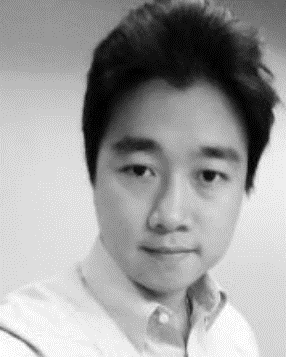
\includegraphics[width=1in,height=1.25in,clip,keepaspectratio]{Figures/bio-li.png}}]%
{Li Zheng}
received the B.S. degree from Zhejiang
University, Hangzhou, China, in 2006, and the dual
M.S. degree in electrical and computer engineering
from Shanghai Jiao Tong University, Shanghai,
China, and the Georgia Institute of Technology,
Atlanta, GA, USA, in 2009, where he is currently
pursuing the Ph.D. degree in electrical and computer
engineering.
His current research interests include embedded
microfluidic cooling, power delivery modeling
and chip-to-chip signaling modeling for high performance
2.5D and 3D systems.
\end{IEEEbiography}


\vspace{-0.3in}


\begin{IEEEbiography}[{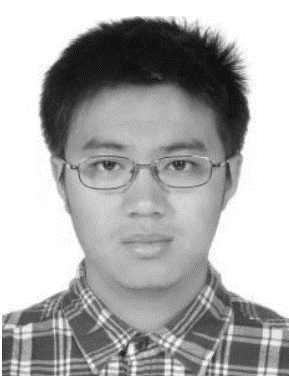
\includegraphics[width=1in,height=1.25in,clip,keepaspectratio]{Figures/bio-yang.png}}]%
{Yang Zhang}
(S�13) received the B.S. degree
in microelectronics and mathematics from Peking
University, Beijing, China, in 2012. He is currently
pursuing the Ph.D. degree in electrical engineering
with the Georgia Institute of Technology, Atlanta,
GA, USA.
\end{IEEEbiography}

\vspace{-0.3in}


\begin{IEEEbiography}[{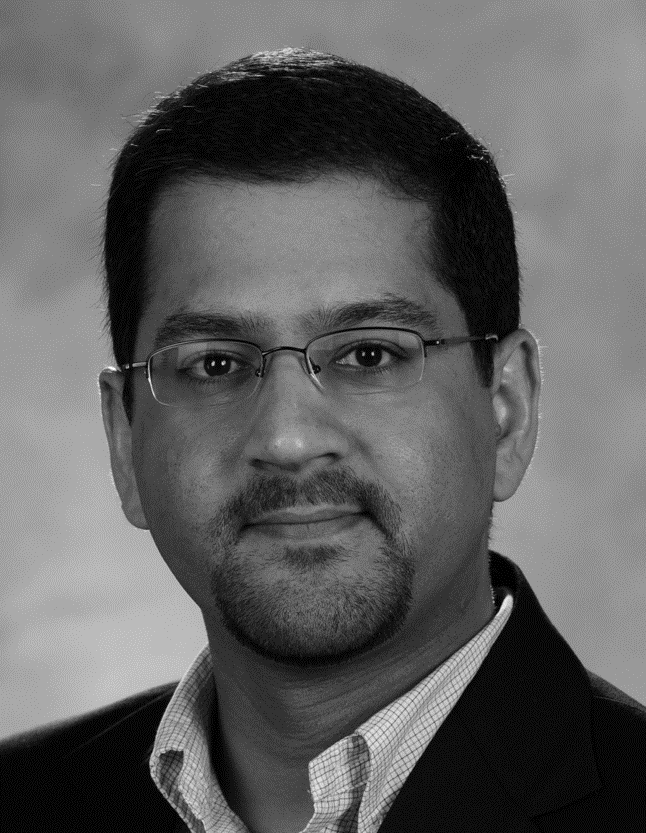
\includegraphics[width=1in,height=1.25in,clip,keepaspectratio]{Figures/bio-muhannad-2b.png}}]%
{Muhannad S. Bakir}
Muhannad S. Bakir (SM'12) received the B.E.E. degree from Auburn University, Auburn, AL, in 1999 and the M.S. 
and Ph.D. degrees in electrical and computer engineering from the Georgia Institute of Technology
in 2000 and 2003, respectively. 
He is currently an Associate Professor in the School of Electrical and Computer Engineering at Georgia Tech. 
His areas of interest include 3D electronic system integration, advanced cooling and power 
delivery for 3D systems, biosensors and their integration with CMOS circuitry, and nanofabrication technology. 
Dr. Bakir is the recipient of the 2013 Intel Early Career Faculty Honor Award, 2012 DARPA Young Faculty Award, 
2011 IEEE CPMT Society Outstanding Young Engineer Award, and was an Invited Participant in the 2012 National 
Academy of Engineering Frontiers of Engineering Symposium. In 2015, Dr. Bakir was elected by the IEEE CPMT 
Society to serve as a Distinguished Lecturer and was an invited speaker at the US National Academies Frontiers 
of Sensor Science Symposium. Dr. Bakir and his research group have received more than fifteen conference and 
student paper awards.
%including five from the IEEE Electronic Components and Technology Conference (ECTC), four 
%from the IEEE International Interconnect Technology Conference (IITC), and one from the IEEE Custom Integrated 
%Circuits Conference (CICC). 
Dr. Bakir's group was awarded the 2014 Best Paper of the IEEE Transactions on 
Components Packaging and Manufacturing Technology in the area of advanced packaging. 
Dr. Bakir is an Editor of IEEE Transactions on Electron Devices and an Associate Editor of IEEE Transactions 
on Components, Packaging and Manufacturing Technology. 
\end{IEEEbiography}

%\vspace{-0.3in}

\vfill


\end{document}

